% Slide 3 — Heterogeneidade da demanda
\begin{frame}{Heterogeneidade da demanda}
  \begin{columns}[T,onlytextwidth]
    \column{0.46\textwidth}
      \textbf{Produto regular}\\
      \small Vende com previsibilidade (ex.: 50 un./semana em qualquer loja).
      \vspace{0.8em}

      \textbf{Produto intermitente / \textit{lumpy}}\\
      \small Períodos de demanda nula intercalados com picos esporádicos
      (ex.: ``0, 0, 0, 50, 0, 0, 30'').
    \column{0.5\textwidth}
      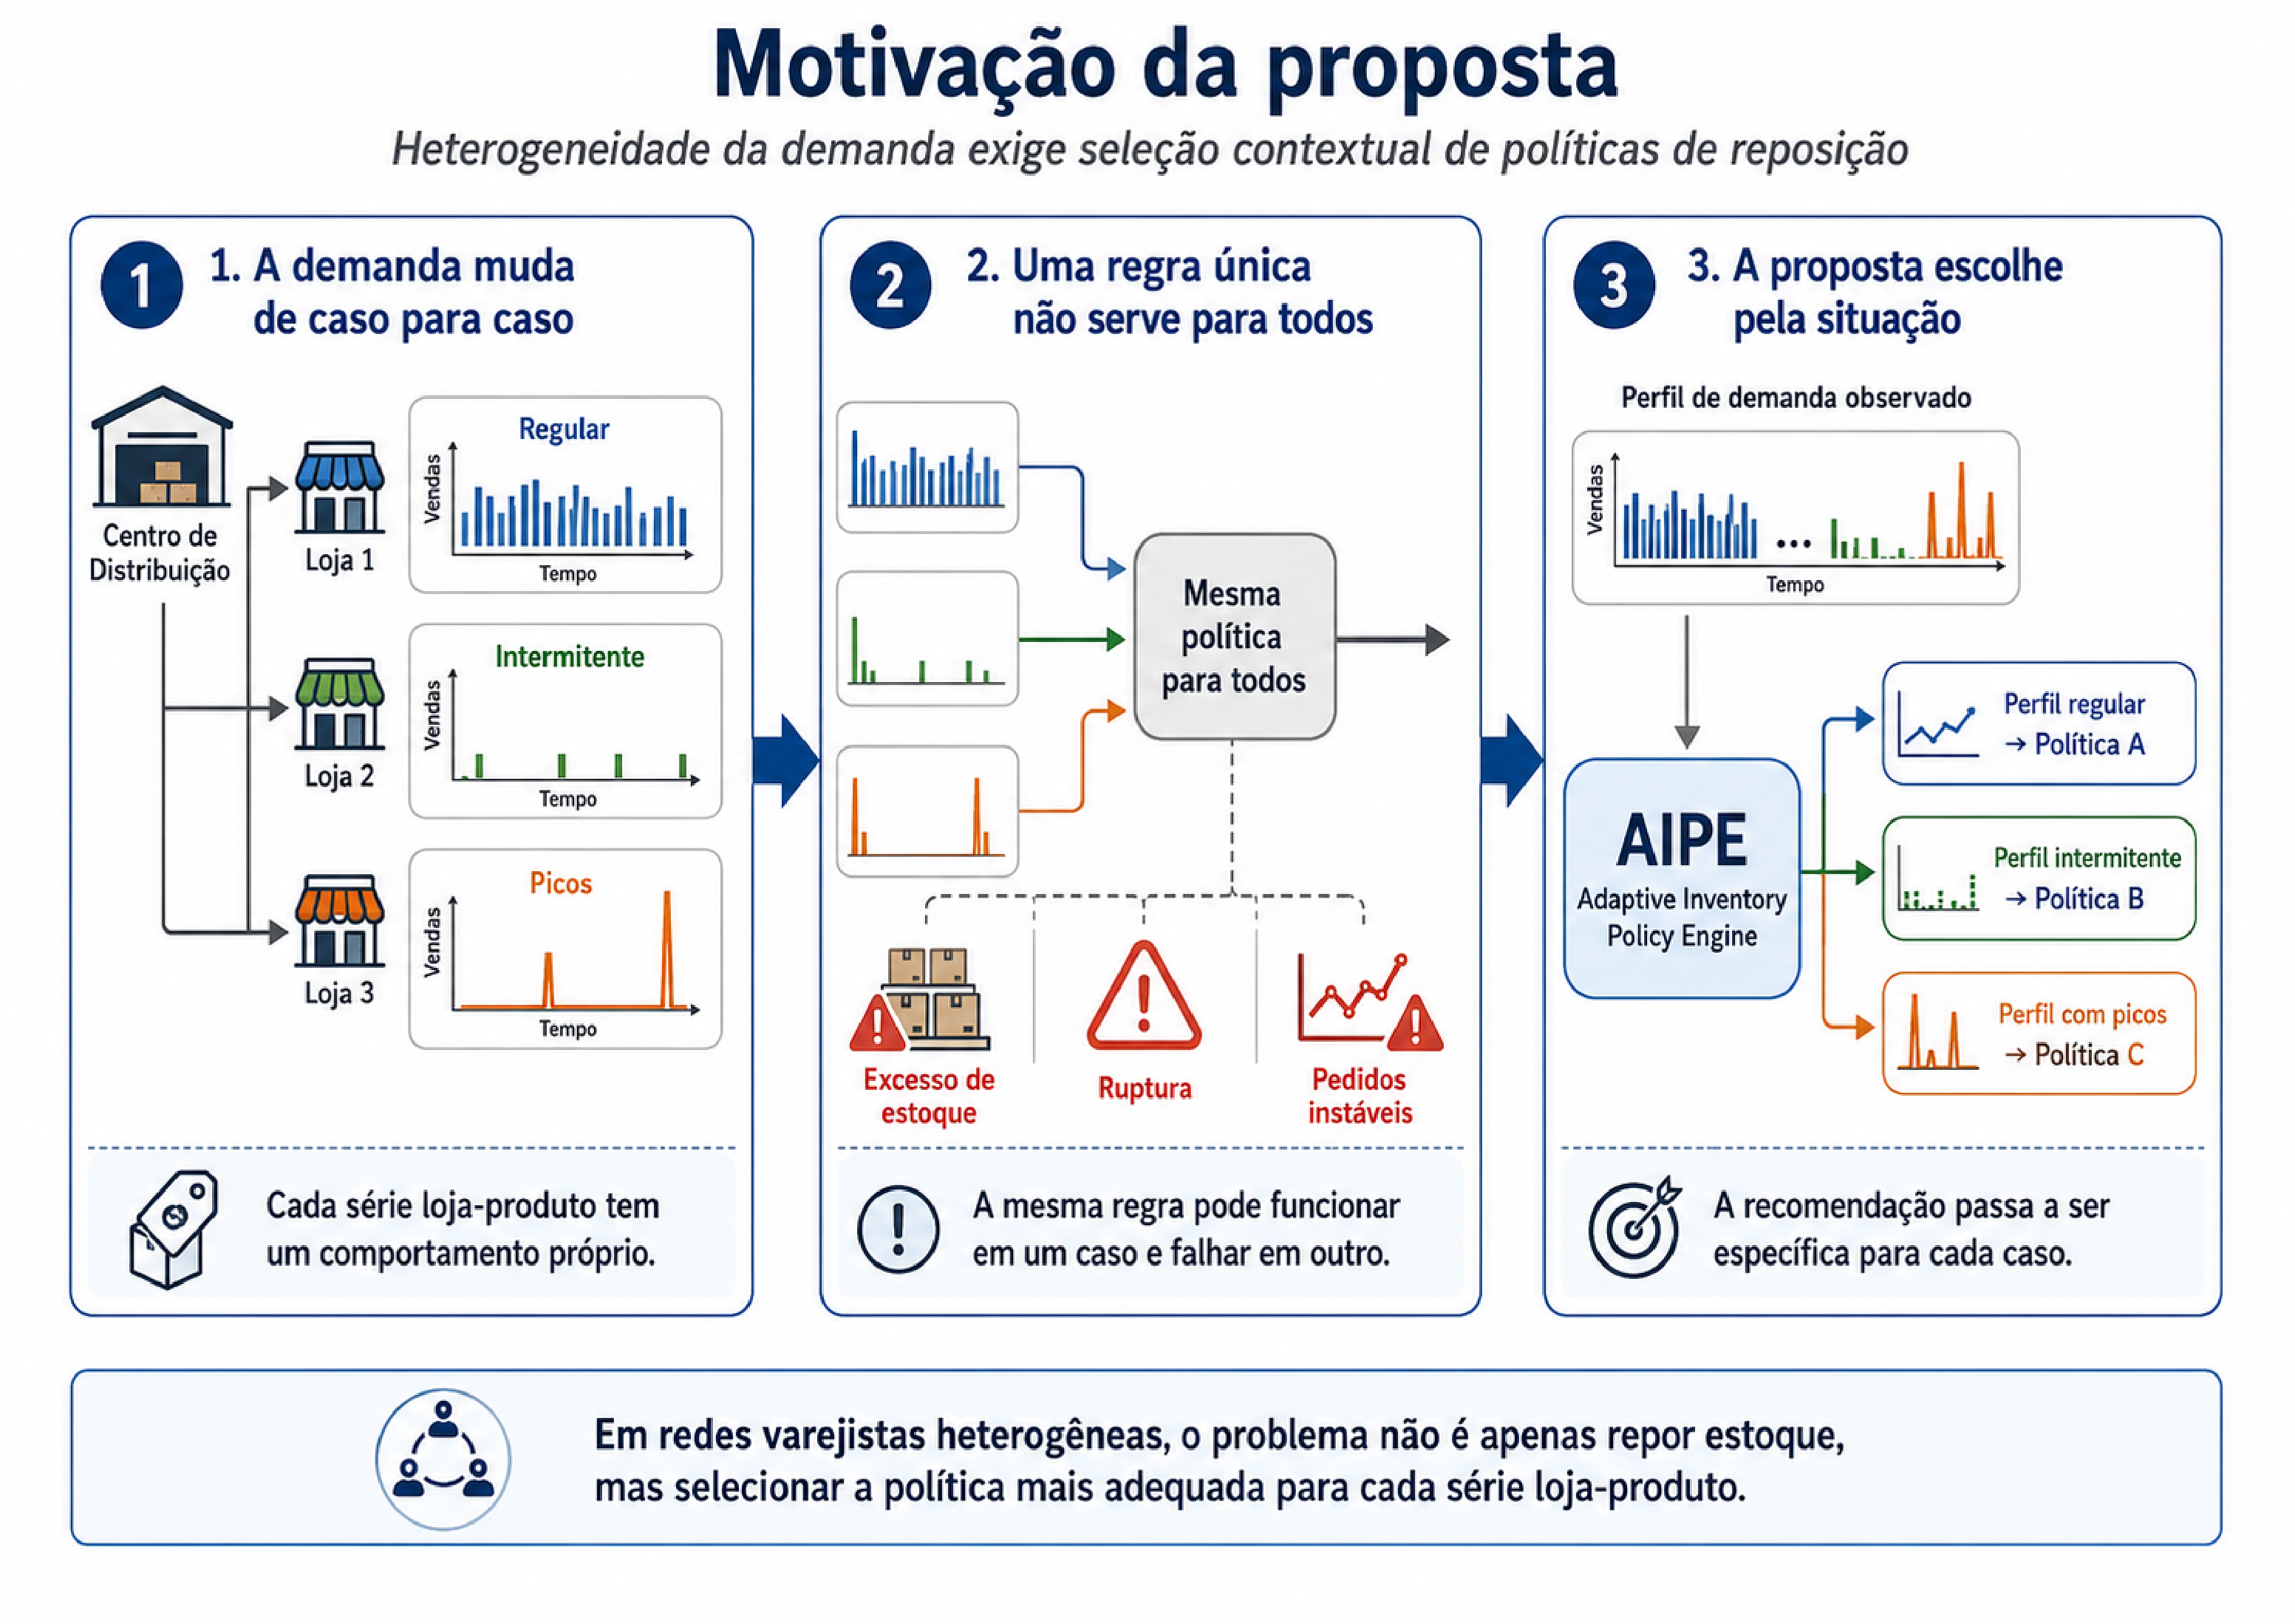
\includegraphics[width=\linewidth,height=4.6cm,keepaspectratio]{figures/figura_1_1_motivacao_aipe.pdf}
  \end{columns}
  \vfill
  \begin{alertblock}{Mesma rede, padrões distintos}
    \small Aplicar a \highlight{mesma política} a séries com comportamentos tão
    diferentes tende a ser ineficiente.
  \end{alertblock}
  \note{
    O ponto central aqui é visual: dentro da mesma rede varejista, produtos
    diferentes (ou o mesmo produto em lojas diferentes) podem ter padrões de
    venda completamente distintos. Uns vendem de forma regular e previsível;
    outros têm longos períodos sem nenhuma venda, seguidos de picos grandes
    e irregulares — isso é o que a literatura chama de demanda intermitente
    ou \textit{lumpy}. Essa figura, que está no Capítulo 1 da dissertação,
    ilustra exatamente essa heterogeneidade que motiva todo o trabalho.
  }
\end{frame}
